\documentclass[11pt,a4paper]{article}

\usepackage[utf8]{inputenc}
\usepackage[T1]{fontenc}
\usepackage[a4paper,margin=2.3cm]{geometry}
\usepackage{graphicx}
\usepackage{booktabs}
\usepackage{float}
\usepackage{array}
\usepackage{amsmath}
\usepackage{amssymb}
\usepackage{hyperref}

\graphicspath{{figures/}}
\hypersetup{
    colorlinks=true,
    linkcolor=blue,
    urlcolor=blue
}

\title{MemristorML\\Project Documentation and Work Log}
\author{Nikola Bari\v{s}i\'{c}}
\date{Updated: 9 September 2026}

\begin{document}

\maketitle
\tableofcontents
\newpage

\section{Project objective}

The project investigates whether switching characteristics of a memristor can
be predicted from measurements available earlier in the device's switching
sequence. The first phase studies the same-cycle mapping

\[
X_{\mathrm{SET},n}
\longrightarrow
Y_{\mathrm{RESET},n},
\]

where both vectors contain

\[
[V_{\mathrm{start}},V_{\mathrm{final}},G_{\mathrm{initial}},
G_{\mathrm{final}}].
\]

The second phase introduces a one-step temporal mapping:

\[
X_{\mathrm{RESET},n}
\longrightarrow
Y_{\mathrm{SET},n+1}.
\]

Linear regression is used as an interpretable baseline before introducing a
small multi-output multilayer perceptron (MLP). Chronological and random data
splits are treated as different experimental protocols rather than as simple
reorderings of the same training rows.

\section{Dataset}

The experiments use \texttt{F2s\_7\_0.parquet}. The dataset contains 5695
cycles and 19 extracted switching metrics. Its columns form a Pandas
MultiIndex with separate \texttt{SET} and \texttt{RESET} groups. Each row is
indexed by the experimental conditions, device identifier, and cycle number:
\texttt{RESET\_pw}, \texttt{RESET\_target}, \texttt{Device}, and
\texttt{Cycle}.

\subsection{Selected inputs and targets}

Both prediction tasks use the following four quantities on each side:

\begin{center}
\begin{tabular}{ll}
\toprule
Input features & Target quantities \\
\midrule
\texttt{start\_v}   & \texttt{start\_v} \\
\texttt{final\_v}   & \texttt{final\_v} \\
\texttt{initial\_g} & \texttt{initial\_g} \\
\texttt{final\_g}   & \texttt{final\_g} \\
\bottomrule
\end{tabular}
\end{center}

Voltage quantities are reported in volts (V), and conductance quantities are
reported in siemens (S).

\section{Data validation and filtering}

Filtering considers only the quantities used by a given model and their
relevant \texttt{has\_error} flags. Missing values in unused metrics do not
cause a cycle to be discarded.

For the same-cycle task, a row is valid only when all four SET inputs, all four
RESET targets, and both error flags are valid.

\begin{table}[H]
\centering
\caption{Dataset validation for the same-cycle task.}
\begin{tabular}{lr}
\toprule
Item & Number of cycles \\
\midrule
Initial dataset & 5695 \\
\texttt{has\_error=True} & 0 \\
Unique cycles with NaN in $X$ or $Y$ & 9 \\
Valid cycles after filtering & 5686 \\
\bottomrule
\end{tabular}
\end{table}

After filtering, both $X$ and $Y$ have shape $5686\times4$, have identical
indices, and contain no remaining NaN values.

\section{Linear regression baseline}

The baseline is a multi-output \texttt{LinearRegression} model from
scikit-learn. Input features are standardized with \texttt{StandardScaler}.
The scaler is fitted on the training inputs, and the learned transformation is
then applied to validation and test inputs.

For a standardized input vector $z$, the model predicts

\[
\hat{y}=Wz+b,
\]

where $W\in\mathbb{R}^{4\times4}$ and $b\in\mathbb{R}^{4}$. Each target has
its own linear combination of the four inputs. The four output regressions are
mathematically independent, although scikit-learn fits them through one
multi-output model call.

Evaluation is reported separately for every target. The metrics used during
the project are mean absolute error (MAE), mean squared error (MSE), root mean
squared error (RMSE), and the coefficient of determination $R^2$.

\section{Phase I: same-cycle SET to RESET prediction}

\subsection{Experiment A: chronological split}

The chronological split preserves the temporal order. The model is fitted on
earlier cycles, validated on the middle portion, and tested on later cycles.

\begin{table}[H]
\centering
\caption{Chronological 80/10/10 split for the same-cycle task.}
\begin{tabular}{lrr}
\toprule
Subset & Number of examples & Cycles \\
\midrule
Train & 4548 & 0--4556 \\
Validation & 569 & 4557--5125 \\
Test & 569 & 5126--5694 \\
\bottomrule
\end{tabular}
\end{table}

\subsubsection{Results}

\begin{table}[H]
\centering
\caption{Same-cycle linear regression on the chronological test set.}
\begin{tabular}{lrrr}
\toprule
RESET target & MAE & RMSE & $R^2$ \\
\midrule
\texttt{start\_v}   & $0.08443$ V & $0.11645$ V & $0.83043$ \\
\texttt{final\_v}   & $0.23417$ V & $0.30350$ V & $0.49526$ \\
\texttt{initial\_g} & $1.3716\times10^{-6}$ S & $1.8907\times10^{-6}$ S & $0.99901$ \\
\texttt{final\_g}   & $8.6023\times10^{-7}$ S & $1.0905\times10^{-6}$ S & $-0.02818$ \\
\bottomrule
\end{tabular}
\end{table}

\begin{figure}[H]
\centering
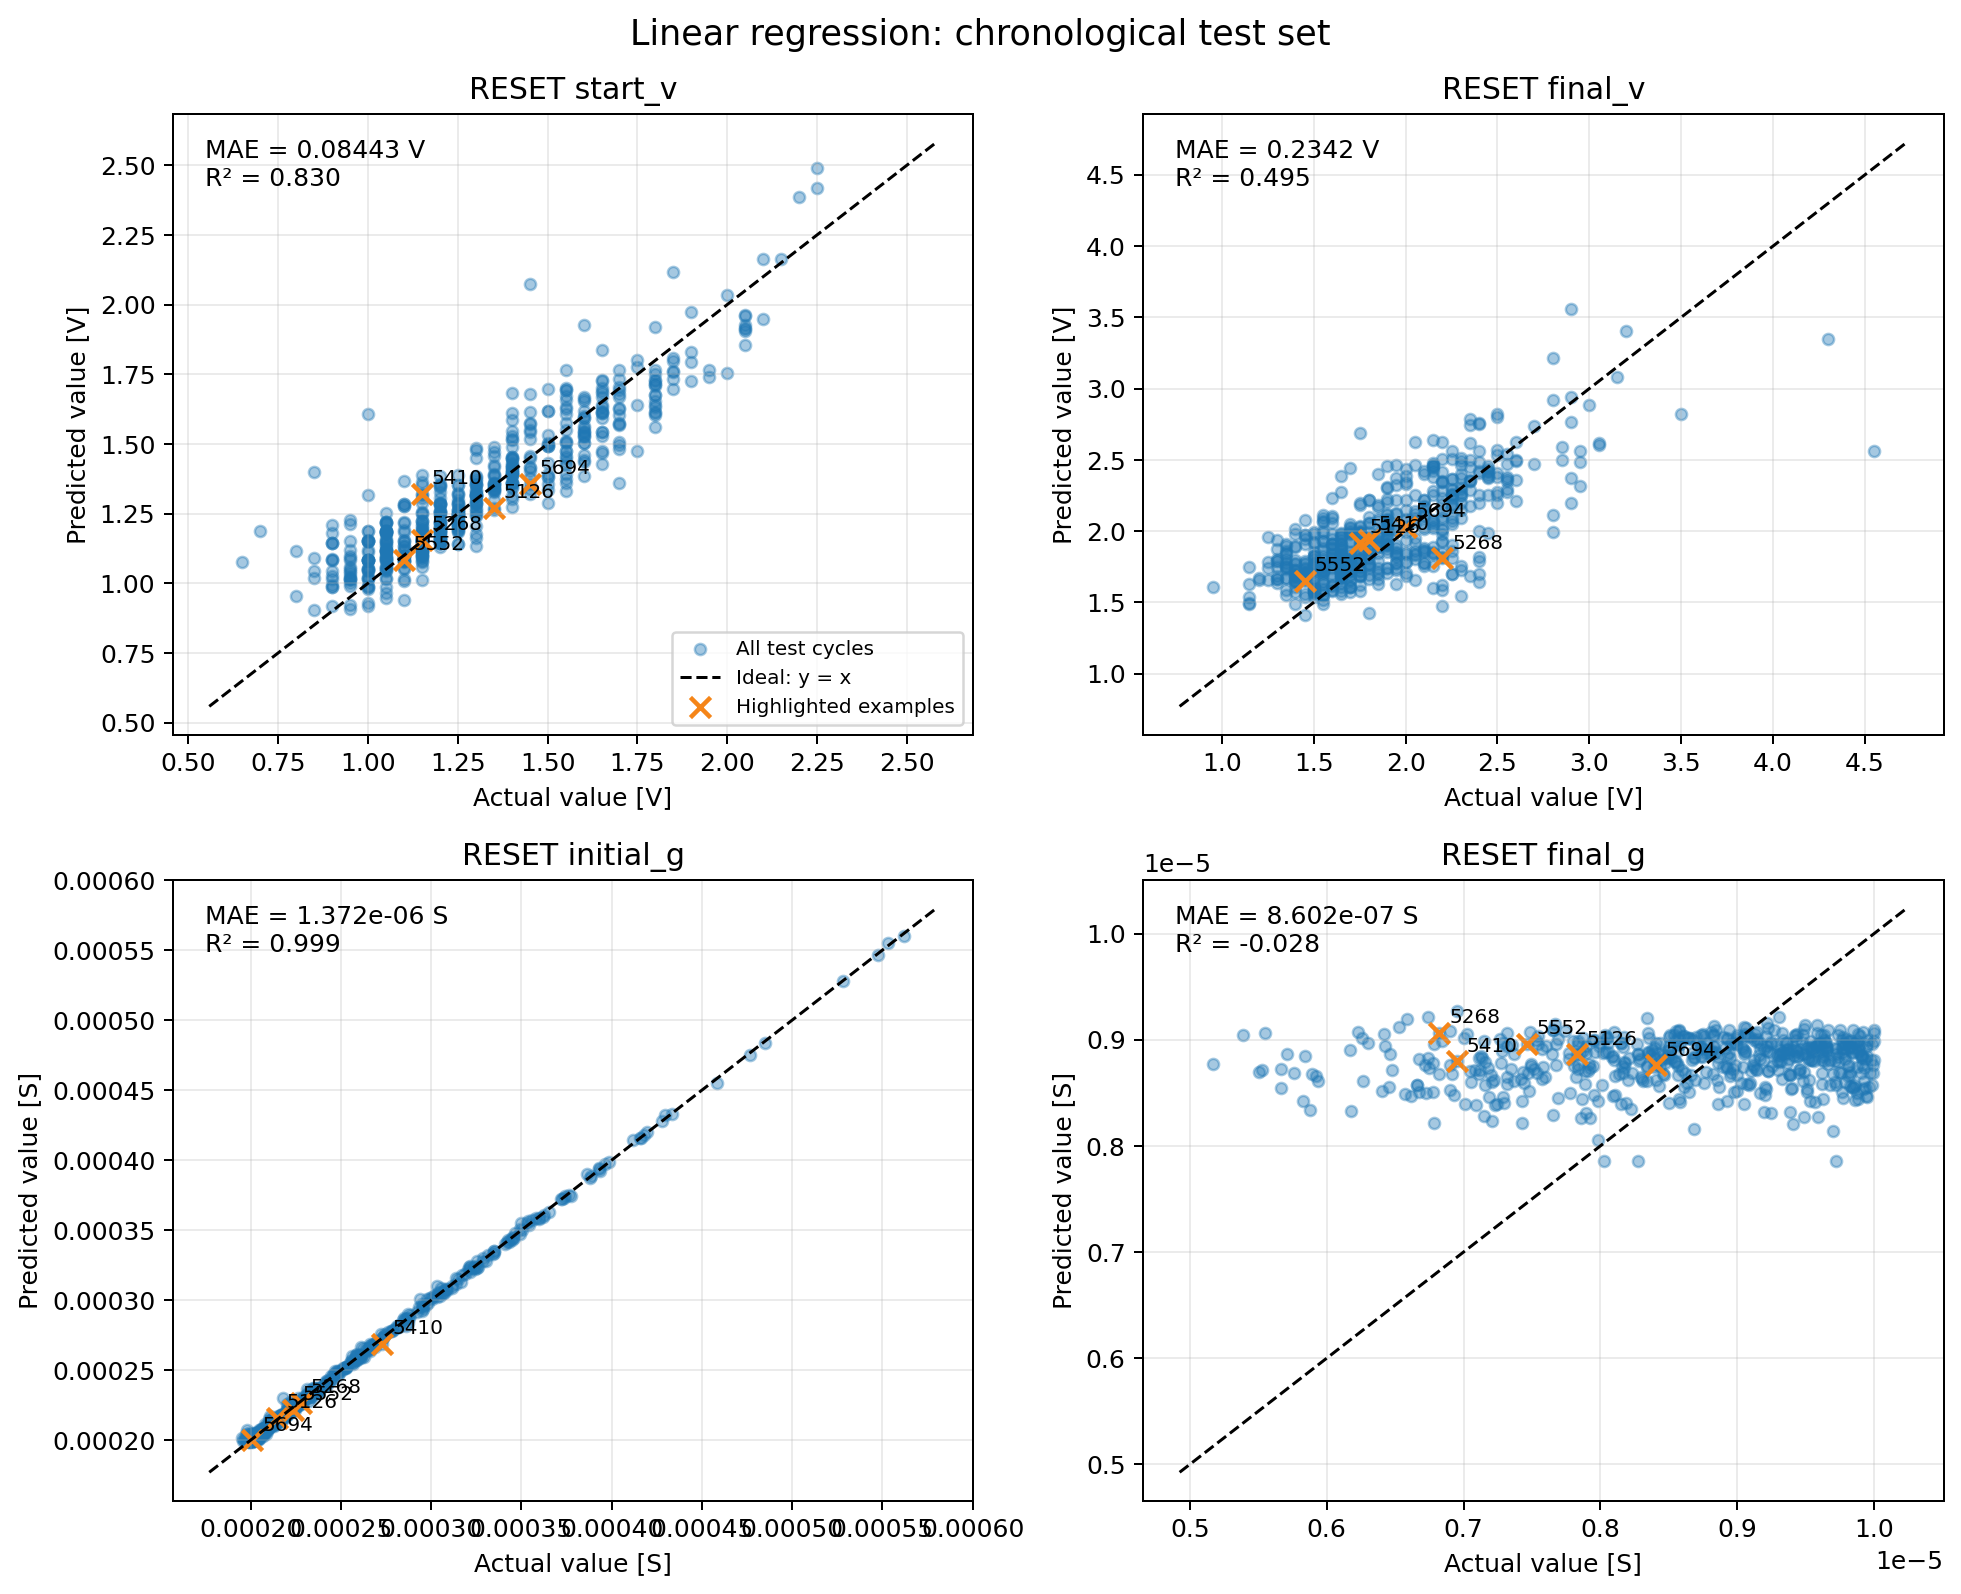
\includegraphics[width=0.98\textwidth]{linear_regression_chronological_predictions.png}
\caption{Actual and predicted RESET values on the chronological test set.}
\label{fig:chronological-predictions}
\end{figure}

\subsubsection{Interpretation}

\texttt{start\_v} has a strong linear signal, whereas \texttt{final\_v} is
only partially predictable. The almost perfect result for
\texttt{initial\_g} is not sufficient evidence of model quality because the
device physics gives the approximate relation

\[
G_{\mathrm{final,SET}}
\approx
G_{\mathrm{initial,RESET}}.
\]

Directly copying \texttt{SET final\_g} to \texttt{RESET initial\_g} already
gives $R^2=0.99866$ on the chronological test set. For \texttt{final\_g}, the
linear model mostly predicts values close to the mean and does not track the
cycle-to-cycle variation.

\subsection{Experiment B: random split}

The same valid dataset is split randomly in an 80/10/10 ratio with
\texttt{random\_state=42}. Each subset contains cycles drawn from the full
temporal range. The subset sizes remain 4548 training, 569 validation, and 569
test examples.

\subsubsection{Results}

\begin{table}[H]
\centering
\caption{Same-cycle linear regression on the random test set.}
\begin{tabular}{lrrr}
\toprule
RESET target & MAE & RMSE & $R^2$ \\
\midrule
\texttt{start\_v}   & $0.08275$ V & $0.12034$ V & $0.75566$ \\
\texttt{final\_v}   & $0.17890$ V & $0.25051$ V & $0.55087$ \\
\texttt{initial\_g} & $1.5293\times10^{-6}$ S & $2.1807\times10^{-6}$ S & $0.99944$ \\
\texttt{final\_g}   & $6.9224\times10^{-7}$ S & $8.8683\times10^{-7}$ S & $0.05883$ \\
\bottomrule
\end{tabular}
\end{table}

\begin{figure}[H]
\centering
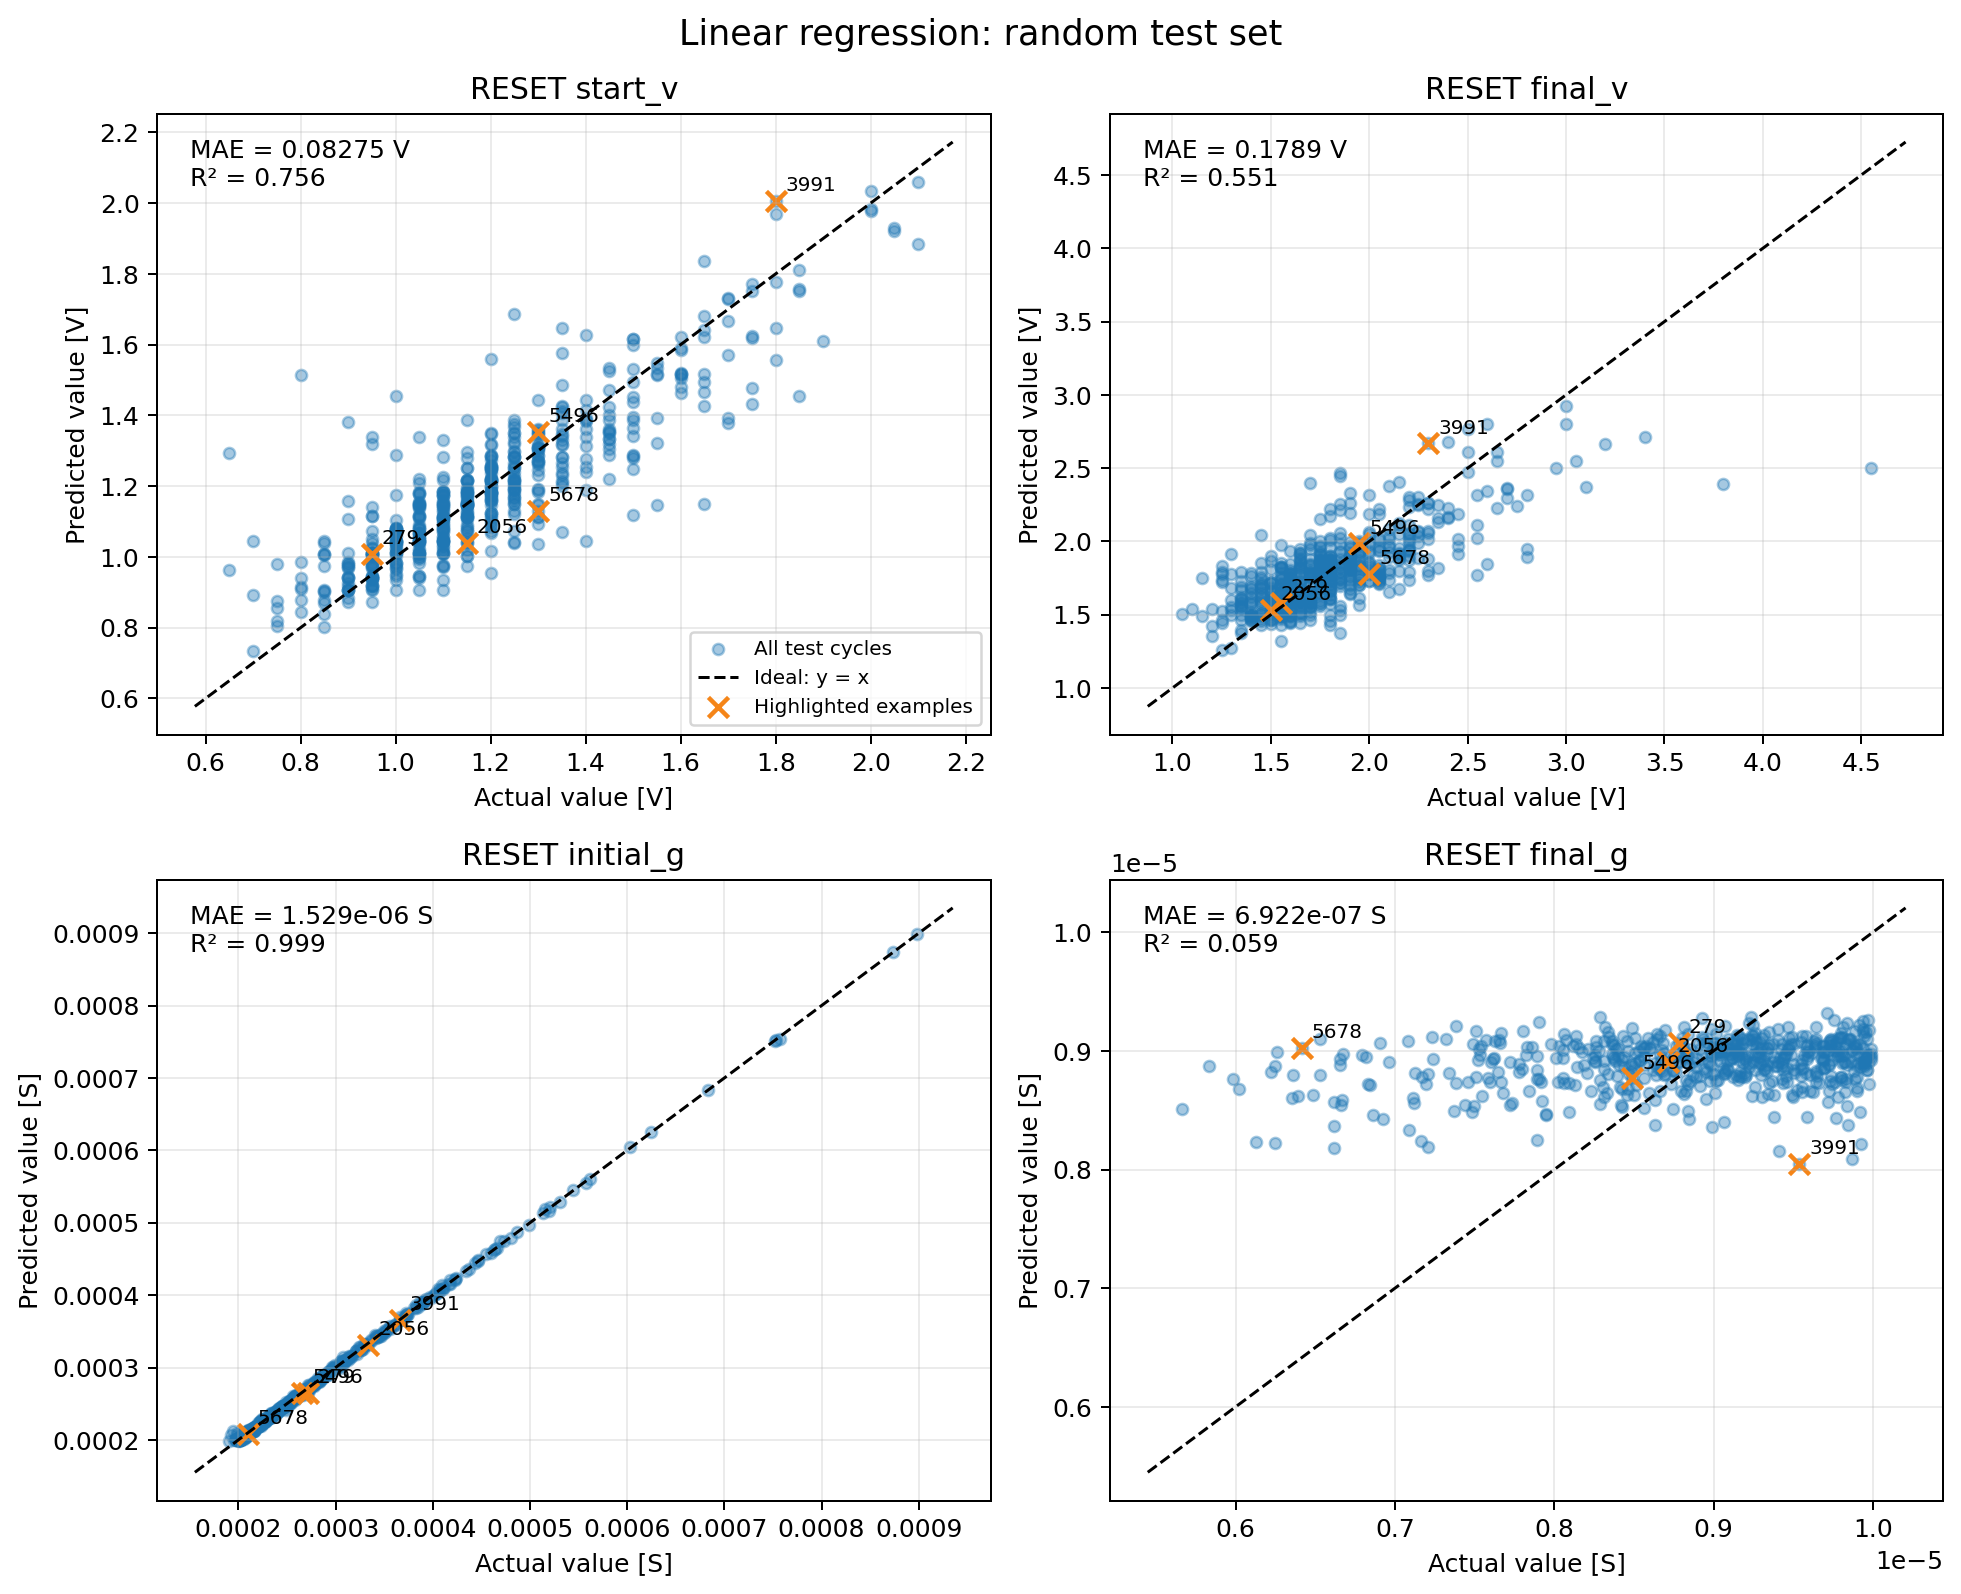
\includegraphics[width=0.98\textwidth]{linear_regression_random_predictions.png}
\caption{Actual and predicted RESET values on the random test set.}
\label{fig:random-predictions}
\end{figure}

\subsection{Comparison of split protocols}

\begin{table}[H]
\centering
\caption{Chronological and random test results. A negative MAE change means that the random model has a lower error.}
\resizebox{\textwidth}{!}{%
\begin{tabular}{lrrrrr}
\toprule
Target & Chron. MAE & Random MAE & MAE change & Chron. $R^2$ & Random $R^2$ \\
\midrule
\texttt{start\_v}   & $0.08443$ & $0.08275$ & $-1.99\%$ & $0.83043$ & $0.75566$ \\
\texttt{final\_v}   & $0.23417$ & $0.17890$ & $-23.60\%$ & $0.49526$ & $0.55087$ \\
\texttt{initial\_g} & $1.3716\!\times\!10^{-6}$ & $1.5293\!\times\!10^{-6}$ & $+11.50\%$ & $0.99901$ & $0.99944$ \\
\texttt{final\_g}   & $8.6023\!\times\!10^{-7}$ & $6.9224\!\times\!10^{-7}$ & $-19.53\%$ & $-0.02818$ & $0.05883$ \\
\bottomrule
\end{tabular}
}
\end{table}

\begin{figure}[H]
\centering
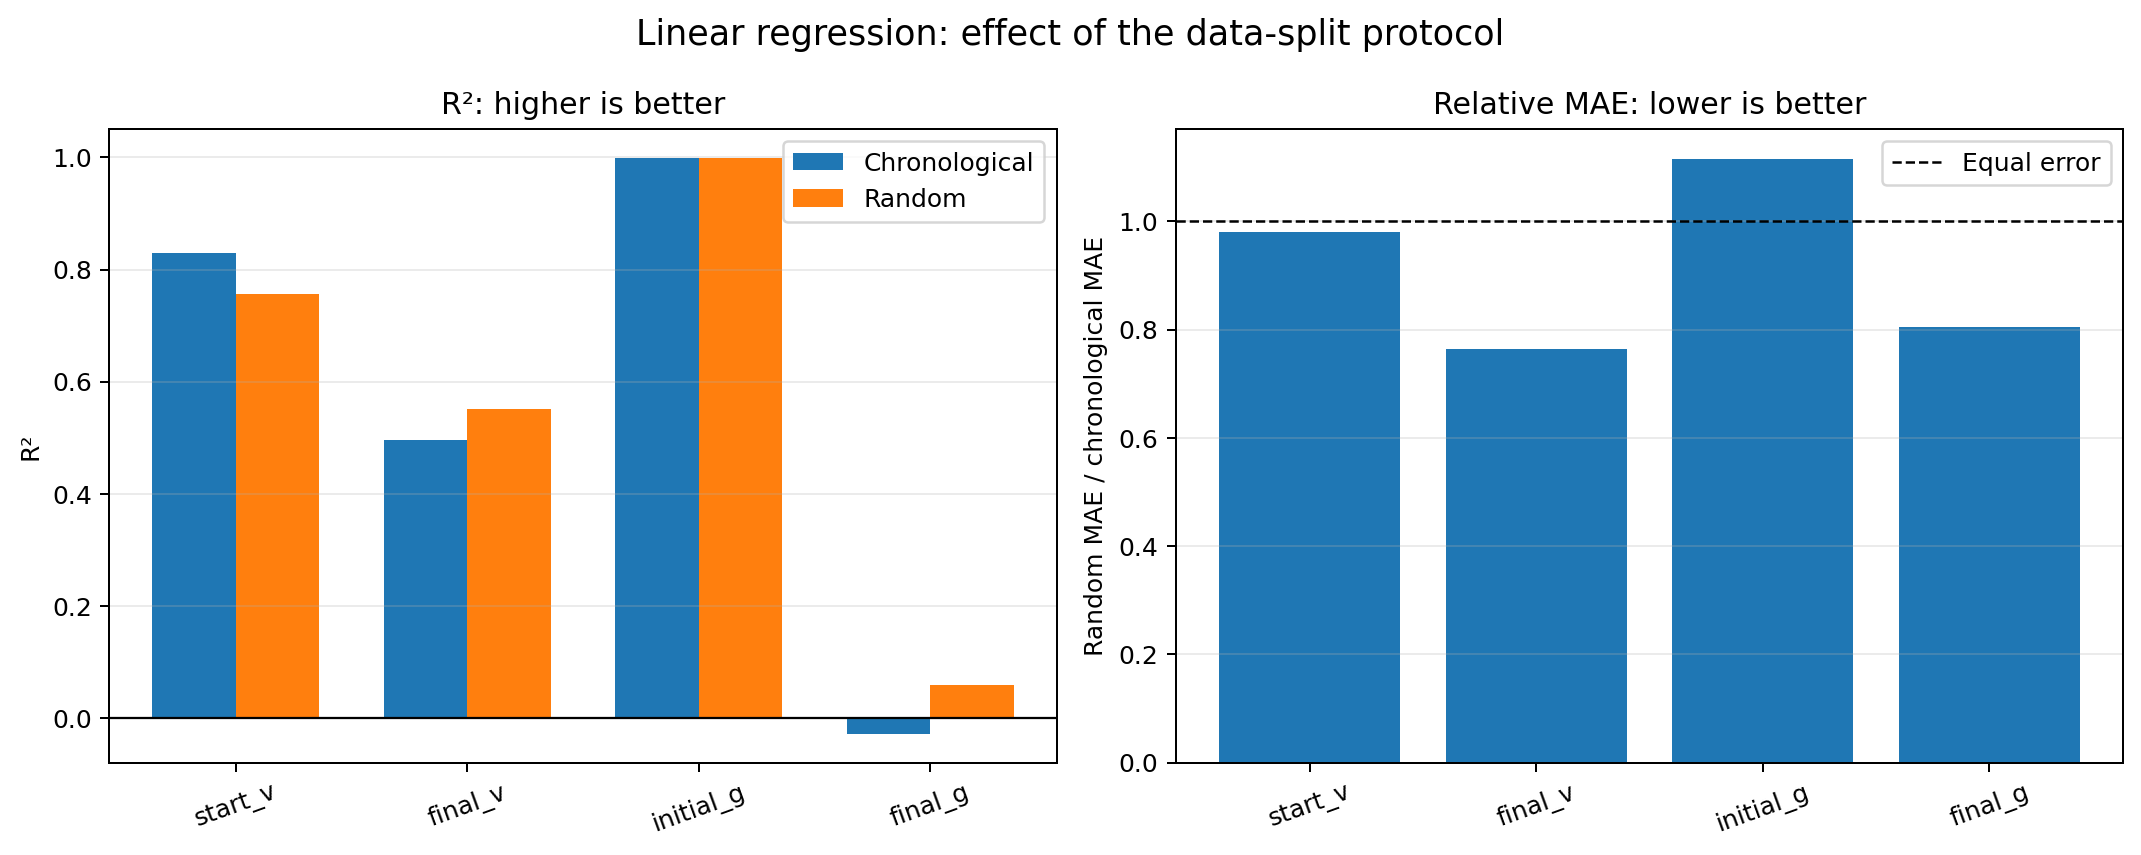
\includegraphics[width=0.98\textwidth]{linear_regression_split_comparison.png}
\caption{Comparison of the chronological and random data-split protocols.}
\label{fig:split-comparison}
\end{figure}

The random split reduces MAE for \texttt{final\_v} by 23.60\% and for
\texttt{final\_g} by 19.53\%. The change for \texttt{start\_v} is small,
whereas \texttt{initial\_g} MAE increases by 11.50\%. These results do not
support a general conclusion that the random protocol is better for every
target. The two test sets contain different cycles and have different target
variances, which also affects $R^2$.

\subsection{Methodological correction: order versus subset composition}

For ordinary linear regression, the order of identical paired training rows
must be distinguished from the composition of the training, validation, and
test subsets. Let $P$ be a permutation matrix that only changes row order:

\[
X'=PX,
\qquad
Y'=PY.
\]

Because $P^TP=I$,

\[
X'^TX'=X^TP^TPX=X^TX
\]

and

\[
X'^TY'=X^TP^TPY=X^TY.
\]

The normal equations, optimal weights, and biases therefore remain unchanged.
The mean and standard deviation used by \texttt{StandardScaler} are also
independent of the order of identical training examples. Only negligible
floating-point differences may occur.

Consequently, the difference between the chronological and random results was
not caused by presenting cycles in a different order. The experiments contain
different members in their training, validation, and test subsets. This
changes the training statistics, $X^TX$, $X^TY$, the fitted parameters, and
the target distribution of the test set. The chronological protocol measures
generalization from earlier to later cycles, whereas the random protocol
measures interpolation among randomly selected cycles of the same device.

\section{Phase II: previous-cycle RESET to next-cycle SET prediction}

The second task predicts the SET characteristics of cycle $n+1$ from the RESET
characteristics of cycle $n$:

\[
\begin{bmatrix}
V_{\mathrm{start}}\\
V_{\mathrm{final}}\\
G_{\mathrm{initial}}\\
G_{\mathrm{final}}
\end{bmatrix}_{\mathrm{RESET},n}
\longrightarrow
\begin{bmatrix}
V_{\mathrm{start}}\\
V_{\mathrm{final}}\\
G_{\mathrm{initial}}\\
G_{\mathrm{final}}
\end{bmatrix}_{\mathrm{SET},n+1}.
\]

\subsection{Temporal pair construction}

RESET inputs are shifted within each experimental group, defined by
\texttt{RESET\_pw}, \texttt{RESET\_target}, and \texttt{Device}. This prevents
the final RESET event of one device or experimental configuration from being
paired with the first SET event of another group. A pair is retained only when
the target cycle is exactly one larger than the input cycle.

\begin{table}[H]
\centering
\caption{Validation of temporal RESET-to-next-SET pairs.}
\begin{tabular}{lr}
\toprule
Item & Number \\
\midrule
Initial rows & 5695 \\
Experimental groups & 1 \\
Rows without a previous RESET cycle & 1 \\
Nonconsecutive candidate pairs & 0 \\
Candidate pairs with NaN values & 14 \\
Candidate pairs with errors & 0 \\
Valid temporal pairs & 5680 \\
\bottomrule
\end{tabular}
\end{table}

Every retained input was independently checked against the raw RESET values of
cycle $n$, and every retained target was checked against the raw SET values of
cycle $n+1$. All 5680 cycle differences are exactly one.

\subsection{Chronological split and model}

\begin{table}[H]
\centering
\caption{Chronological 80/10/10 split for the temporal task.}
\begin{tabular}{lrrr}
\toprule
Subset & Examples & RESET input cycles & SET target cycles \\
\midrule
Train & 4544 & 0--4557 & 1--4558 \\
Validation & 568 & 4558--5125 & 4559--5126 \\
Test & 568 & 5126--5693 & 5127--5694 \\
\bottomrule
\end{tabular}
\end{table}

The model uses the same \texttt{StandardScaler} and multi-output linear
regression pipeline as Phase I. The input scaler is fitted on the 4544 training
pairs. Targets remain in their original physical units.

\subsection{Test results}

Relative MAE is defined as

\[
\mathrm{relative\ MAE}\,[\%]
=100\frac{\mathrm{MAE}}{\operatorname{mean}(|y_{\mathrm{true}}|)}.
\]

This quantity is not MAPE. It avoids dividing separately by potentially tiny
individual conductance values and handles signed voltage targets consistently.

\begin{table}[H]
\centering
\caption{Temporal linear regression on the chronological test set.}
\begin{tabular}{lrrrr}
\toprule
SET target & MSE & RMSE & Relative MAE & $R^2$ \\
\midrule
\texttt{start\_v}   & $0.0381462$ & $0.195311$ V & $11.13\%$ & $0.260043$ \\
\texttt{final\_v}   & $0.0464381$ & $0.215495$ V & $9.77\%$ & $0.585228$ \\
\texttt{initial\_g} & $1.15104\times10^{-12}$ & $1.07286\times10^{-6}$ S & $9.55\%$ & $0.342966$ \\
\texttt{final\_g}   & $3.07647\times10^{-9}$ & $5.54660\times10^{-5}$ S & $14.97\%$ & $0.149403$ \\
\bottomrule
\end{tabular}
\end{table}

MSE has squared target units: V$^2$ for voltage targets and S$^2$ for
conductance targets.

\begin{figure}[H]
\centering
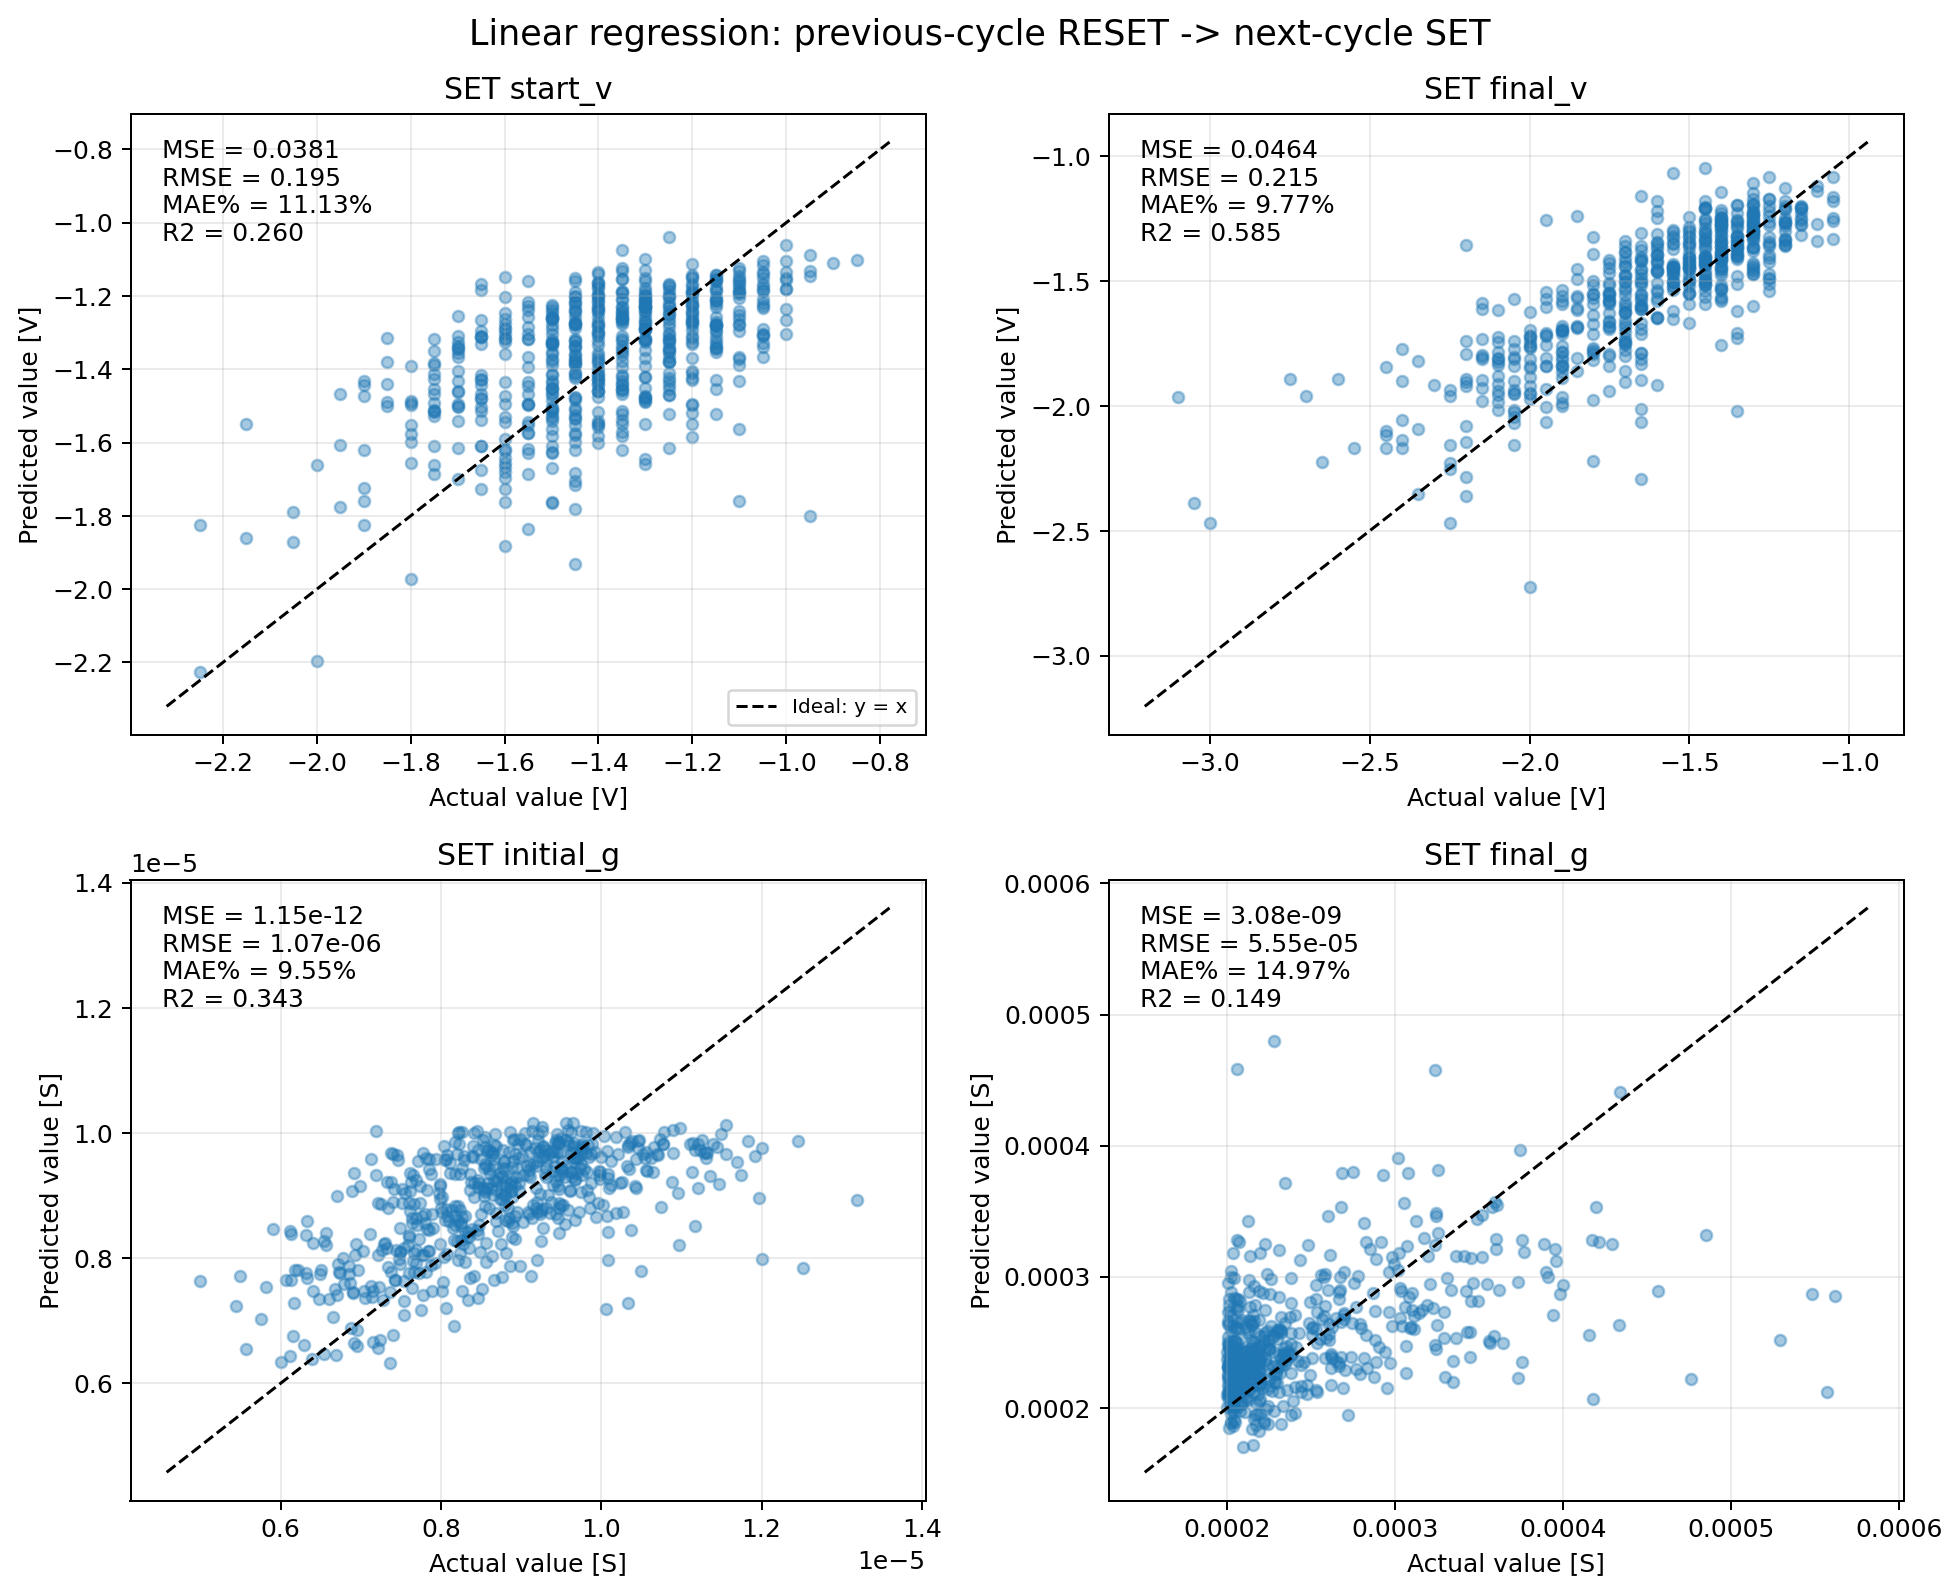
\includegraphics[width=0.98\textwidth]{linear_regression_reset_to_next_set_predictions.png}
\caption{Actual and predicted next-cycle SET values on the chronological test set.}
\label{fig:reset-next-set-predictions}
\end{figure}

\begin{figure}[H]
\centering
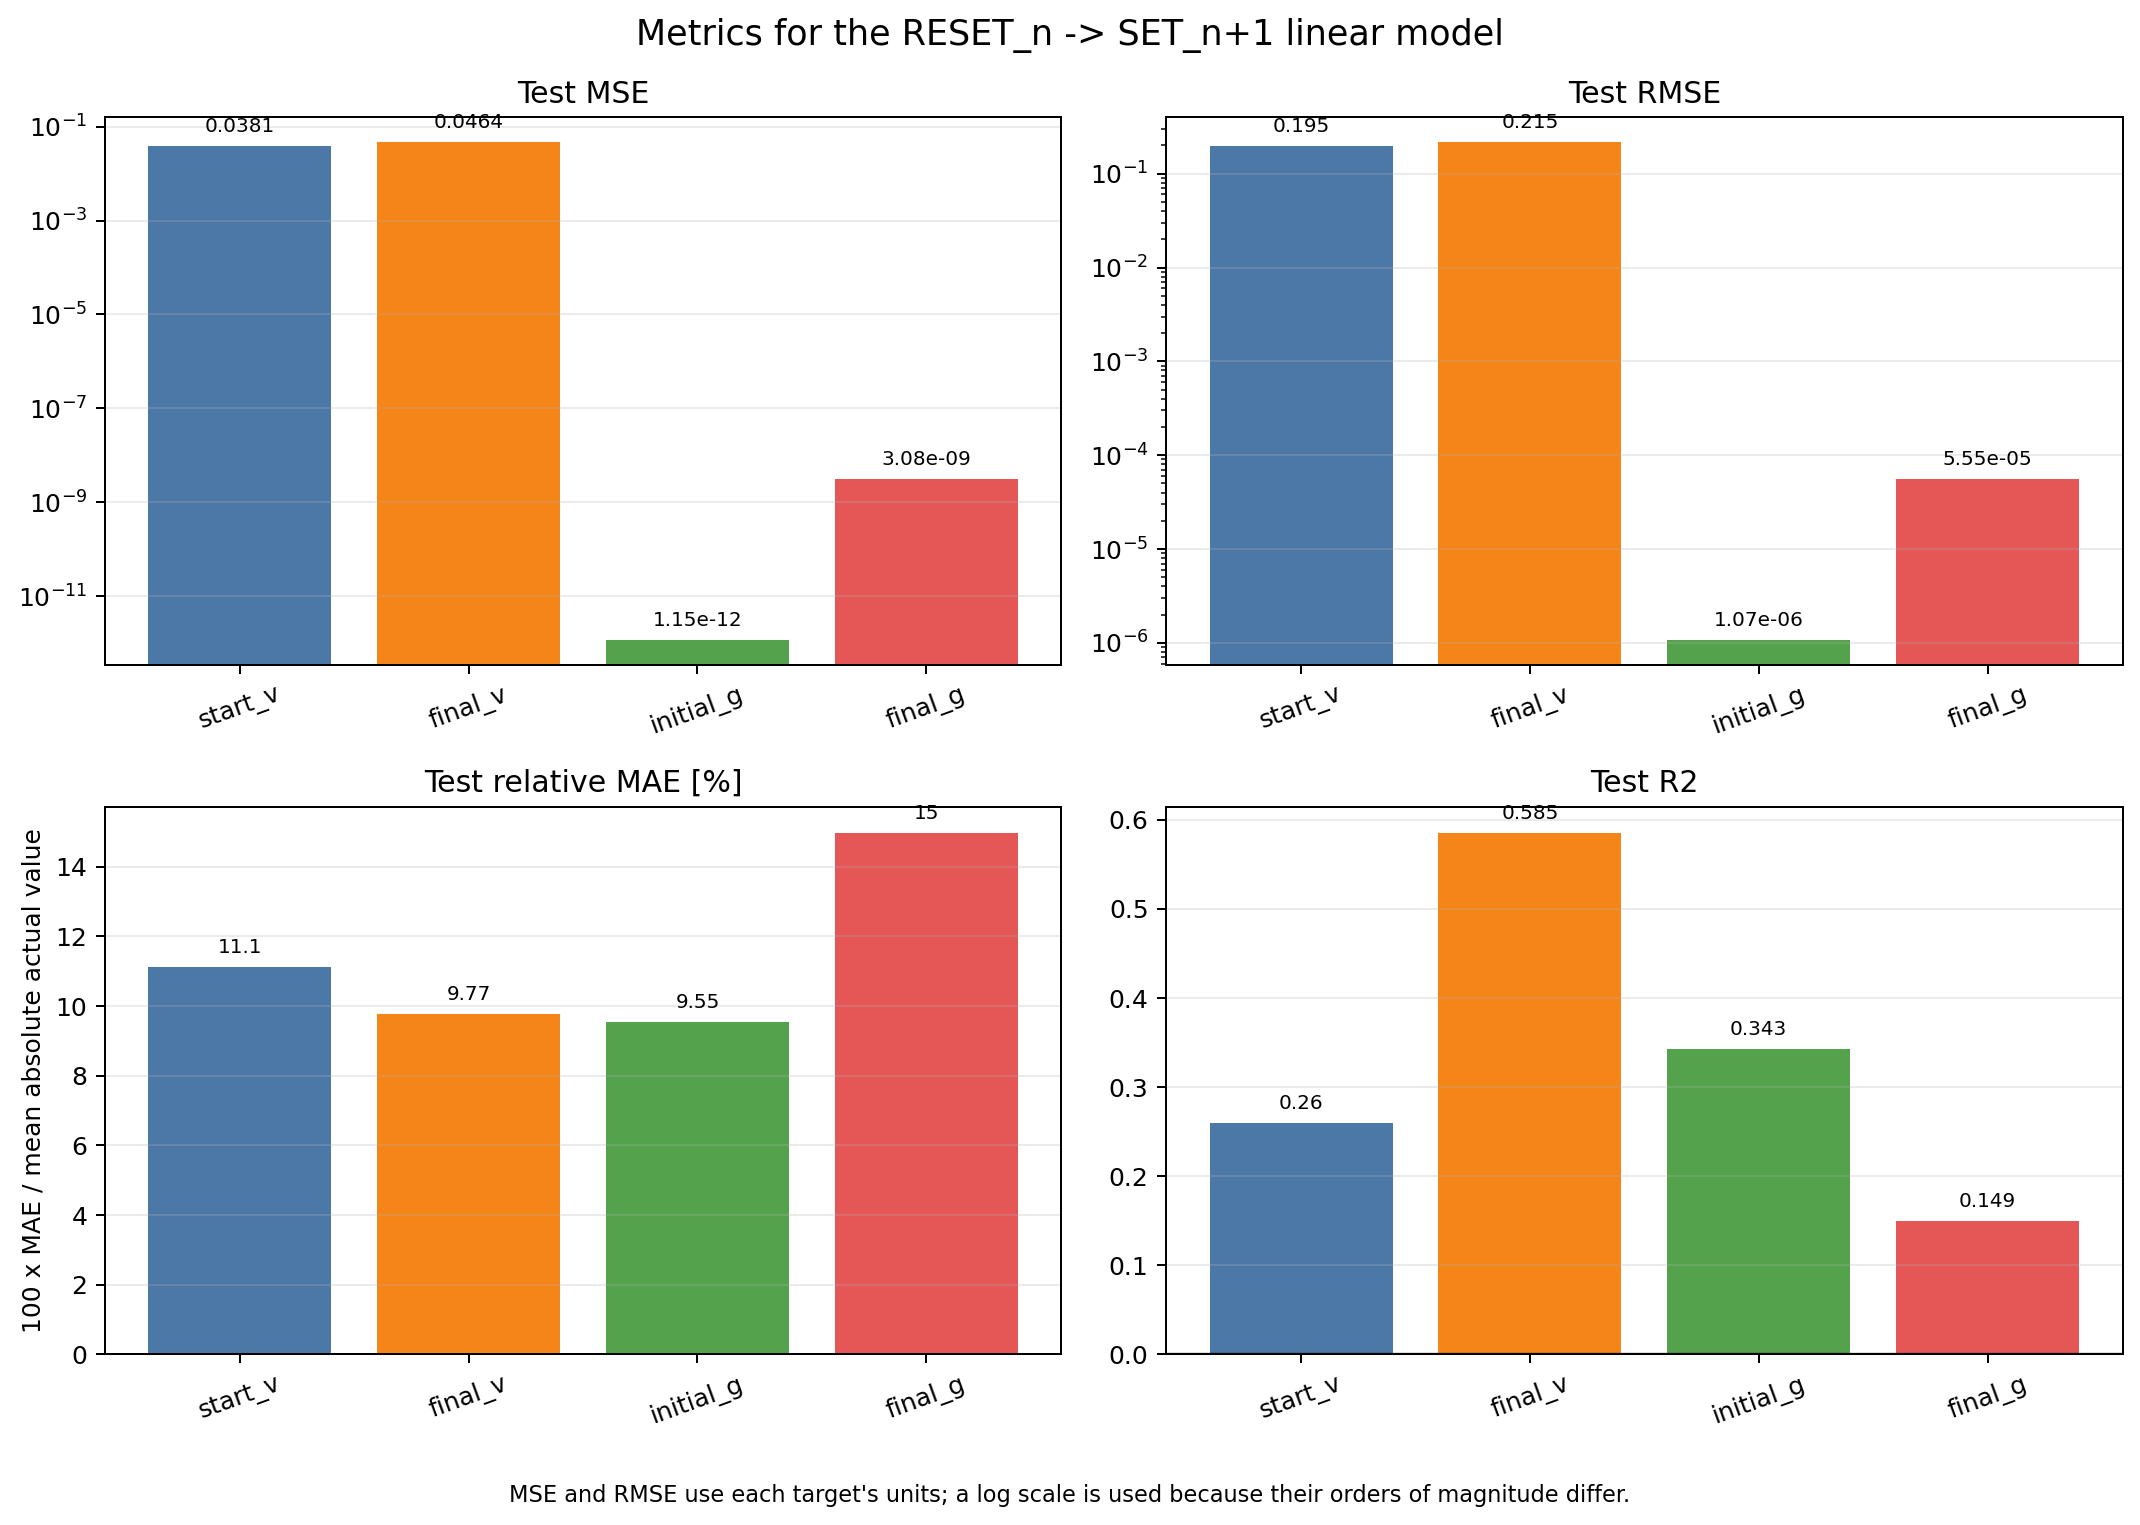
\includegraphics[width=0.98\textwidth]{linear_regression_reset_to_next_set_metrics.png}
\caption{Per-target metrics for the temporal linear regression baseline.}
\label{fig:reset-next-set-metrics}
\end{figure}

\subsection{Interpretation}

Among the four targets, \texttt{final\_v} has the strongest temporal linear
signal, with $R^2=0.585$. The linear model explains less of the variation in
\texttt{start\_v} and \texttt{initial\_g}. The weakest result is obtained for
\texttt{final\_g}, with $R^2=0.149$ and a relative MAE of 14.97\%. The previous
RESET event therefore contains useful information about the next SET event,
but a linear mapping does not explain most of the variation for all targets.
This provides a justified baseline for a later nonlinear MLP experiment.

\section{Decisions}

\begin{itemize}
    \item Metrics are reported separately for every target because voltage and
    conductance use different physical units and scales.
    \item Input scalers are fitted on training inputs only.
    \item Chronological and random protocols remain separate because they
    answer different research questions.
    \item Reordering identical training examples does not change the
    least-squares solution; changing subset membership does.
    \item \texttt{RESET initial\_g} is not used as the main evidence of Phase I
    model quality because of its direct physical relationship with
    \texttt{SET final\_g}.
    \item Temporal pairs are constructed within experimental groups and must
    connect consecutive cycles only.
    \item Relative MAE is reported with its explicit normalization formula and
    is not labelled as MAPE.
    \item Tables and figures accompany every major experiment.
\end{itemize}

\section{Next steps}

\begin{enumerate}
    \item Complete the line-by-line audit of the temporal linear regression
    code and its metrics.
    \item Add a mean baseline and relevant physics-based baselines.
    \item Empirically verify row-order invariance by fitting the same linear
    model before and after permuting identical training pairs.
    \item Repeat the random split with multiple seeds and report the mean and
    standard deviation of every metric.
    \item Implement a small multi-output MLP, initially
    $4\rightarrow16\rightarrow16\rightarrow4$.
    \item Standardize both inputs and targets for the MLP using statistics
    fitted on the training subset.
    \item Select the MLP with the validation subset and early stopping, then
    evaluate the selected configuration once on the test subset.
    \item Compare the MLP with the mean, physics-based, and linear baselines
    under matching split protocols.
    \item Later extend the temporal context beyond one previous RESET event.
\end{enumerate}

\section{Work log}

\begin{description}
    \item[28 August 2026] Loaded and validated the Parquet dataset; defined
    same-cycle SET inputs and RESET targets; formed a valid dataset of 5686
    cycles; implemented a chronological split and multi-output linear
    regression baseline; added metrics, individual test examples, and an
    actual-versus-predicted figure.

    \item[1 September 2026] Implemented a reproducible random 80/10/10 split
    with \texttt{random\_state=42}; fitted the same linear model; created
    numerical and graphical comparisons with the chronological experiment;
    introduced a persistent LaTeX project log.

    \item[3 September 2026] Corrected the interpretation of the random
    experiment after a discussion with the supervisors. Established that
    ordinary least-squares linear regression is invariant to the order of
    identical paired training examples. Added the permutation-matrix proof and
    updated the experimental plan.

    \item[7 September 2026] Implemented the temporal
    $\mathrm{RESET}_n\rightarrow\mathrm{SET}_{n+1}$ dataset construction,
    chronological split, linear regression baseline, per-target metrics, and
    diagnostic figures. Independently verified all 5680 temporal pairs against
    the raw dataset.

    \item[9 September 2026] Converted the source code, plots, and project
    documentation to English and consolidated both prediction tasks in the
    project log.
\end{description}

\end{document}
